\section{Grundlagen}
\label{sec:grundlagen}

In diesem Kapitel gilt es zu klären, auf welchen Grundlagen, Ideen und Konzepten Model-View-Intent beruht, wie diese miteinander fungieren und weshalb sie als Inspiration dienten.

\subsection{Unidirektionaler Datenfluss: Flux, Redux und React}

In einer Applikation existieren grundsätzlich zwei Komponenten: Eine, die der Nutzer wahrnehmen kann und eine, die für ihn unsichtbar bleibt. Bei ersterer handelt es sich meist um das, was der Nutzer(auf dem Bildschirm) sieht - die sogenannte »View«. Die zweite Komponente beschreibt die Ebene, welche das Geschehen observiert, darauf reagiert und den weiteren Verlauft (zum größten Teil) kontrolliert. Sie kann unter anderem als »Controller« betitelt werden.
\\
\\
Der Zustand in dem sich eine Applikation befindet kann hierbei von beiden Seiten modifiziert und beobachtet werden. Ist dies der Fall, so handelt es sich um einen bidirektionalen Datenfluss. Bei dieser Variante entsteht die eventuelle Gefahr von kaskadierenden Updates (ein Objekt verändert ein anderes, welches wiederum eine Veränderung bei einem weiteren herbeiführt usw.) als auch in einen unvorhersehbaren Datenfluss zu geraten: Es wird schwer, den Datenfluss nachzuvollziehen. Des weiteren muss immer überprüft und sichergestellt werden, dass »View« und »Controller« synchronisiert sind, da beide den globalen Zustand darstellen. Schlussendlich verliert man zusätzlich die Fähigkeit zu entscheiden, wann und welcher Stelle der Zustand manipuliert wird.
\\
\\
Ein anderer Ansatz ist, den Datenfluss in eine Richtung zu beschränken und ihn damit unidirektional
\cite{unidirectionalDataFlowFluxArchitectureIlyGelman2017, unidirectionalDataFlowTheCompleteReduxBookIlyGelman2017}
operieren zu lassen. Diese Variante erfreut sich an zunehmender Popularität seit der Bekanntmachung der »Flux«
\cite{fluxArchitectureAdamBoduch}
Architektur im Jahre 2015 von Facebook.
\cite{fluxAnnouncementYoutube}

\subsubsection{Flux}
Für die Einhaltung und Umsetzung eines unidirektionalen Datenfluss bedient sich »Flux« bei zwei fundamentalen Konzepten: Der Zustand innerhalb einer Applikation wird als »single source of truth (SSOT)« angesehen und darf keine direkte Änderung erfahren. Um dies zu Gewährleisten finden sich mehrere Komponenten in »Flux« wieder:
\\
\\
\textbf{Action}: Eine Aktion beschreibt ein Ereignis, welches unter anderem vom Nutzer ausgelöst werden kann. Sie geben vor, wie mit der Anwendung interagiert wird. Jeder dieser Aktionen wird dabei ein Typ zugewiesen. Insgesamt sollte eine Aktion semantisch und deskriptiv bezüglich der Intention sein. Des weiteren können zusätzliche Attribute an eine Aktion gebunden werden.
\\
\\
\begin{lstlisting}[frame=single, language=Java]
{
 type: ActionTypes.INCREMENT,
 by: 2
}
\end{lstlisting}
\space
\textbf{Dispatcher}: Er ist für die Entgegennahme und Verteilung einer Aktion an sogenannte »Stores« zuständig. Diese haben die Möglichkeit sich beim ihm zu registrieren. Er besitzt die wichtige Eigenschaft der sequentiellen Verarbeitung, d.h., dass er zu jedem Zeitpunkt nur eine »Action« weiterreicht. Sämtliche »Stores« werden über alle Aktionen unterrichtet.
\\
\\
\textbf{Store}: Hier befinden sich die Daten, welche einen Teil des globalen Zustands einer Anwendung ausmachen. Die einzige Möglichkeit für eine Veränderung der dort hinterlegten Daten besteht durch ein Reaktion auf eine, vom »Dispatcher« kommenden, Aktion. Bei jeder Modifikation der Daten erfolgt die Aussendung eines Events an eine »View«, das die Veränderung mitteilt.
Ebenso findet sich hier ein Part der Anwendungslogik.
\\
\\
\textbf{View}: Die View ist für die Anzeige und Eingabe von Daten zuständig - sie ist die für den Nutzer sichtbare Komponente, mit welcher dieser interagiert. Ihre Daten erhält sie von einem »Store«, diesen sie abonniert und auf Änderungsereignisse hört. Erhält sie vom »Store« ein solches Änderungsereignis, so kann sie die neuen Daten abrufen und sich selbst aktualisieren. Der View ist es nicht gestattet, den Zustand direkt zu verändern. Stattdessen generiert sie eine Aktion schickt diese an den Dispatcher.
\\
Ein Beispielhafter Ablauf bei einer Anwendung die einen Wert erhöht oder verringert kann wie folgt aussehen:
\begin{enumerate}
	\item Die View bekommt einem Store zugewiesen, welcher für das inkre- und dekrementieren der angezeigten Zahl verantwortlich ist.
	\item Sie erhält die Anfangszahl und stellt diese in einem leserlichen Format/einer Ansicht dar, welches es dem Nutzer ermöglicht, damit zu interagieren.
	\item Betätigt dieser einer der Knöpfe welche die dargestellte Zahl verändern, so wird eine Action erstellt und an Dispatcher geschickt.
	\item Dieser wiederum informiert alle Stores.Information
	\item Jener Store der für die Verarbeitung dieser Aktion verantwortlich ist, modifiziert die Zahl in seiner internen Datenstruktur und kommuniziert dies über ein Änderungsereignis
	\item Diejenige View, welche auf Änderungsereignisse diesen Ursprungs lauscht, erhält die Daten und aktualisiert sich dementsprechend. 
\end{enumerate}
\clearpage
\begin{figure}[ht]
	\centering
	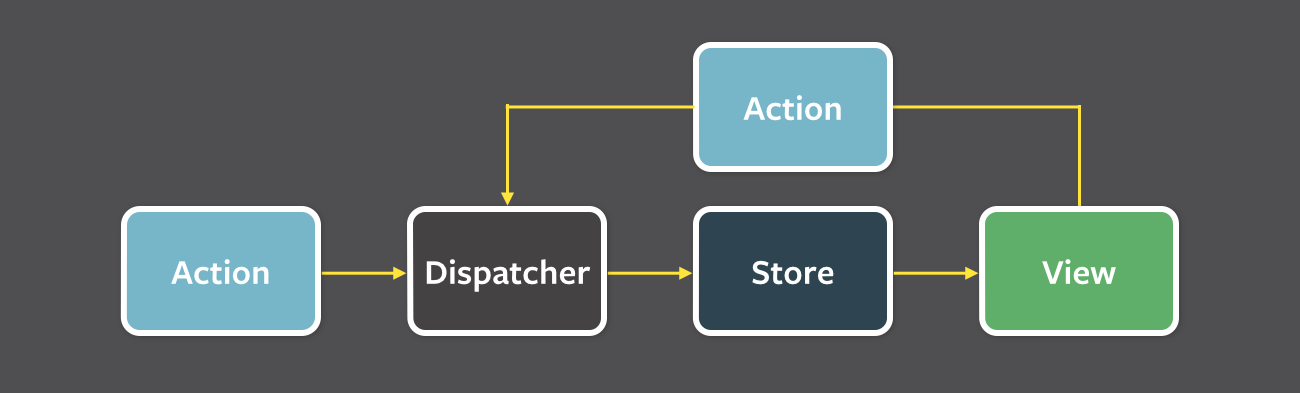
\includegraphics[height=0.25\textwidth]{./images/flux-flow}
	\caption{Datenfluss in der Flux Architektur}
	\label{fig:datenflussFlux}
\end{figure}

Anhand Abbildung \ref{fig:datenflussFlux} wird der unidirektionale Datenfluss deutlich erkennbar:
\begin{enumerate}
	\item Die View schickt eine Aktion an den Dispatcher.
	\item Dieser leitet diese an alle Stores weiter.
	\item Der Store verarbeitet die Daten und informiert die View.
\end{enumerate}





